\documentclass[12pt]{article}
\usepackage[dvips]{graphicx}

\begin{document}
\section{Result}

For the test case in Introduction,we do numerical computation on four meshes:
$$h_{1}=2^{-3}, h_{2}=2^{-4}, h_{3}=2^{-5}, h_{4}=2^{-6}$$

Our permeability is $K(x,y)=\frac{1.0}{2+1.99*sin(2 \pi \frac{2x-y}{\epsilon})}$:\\

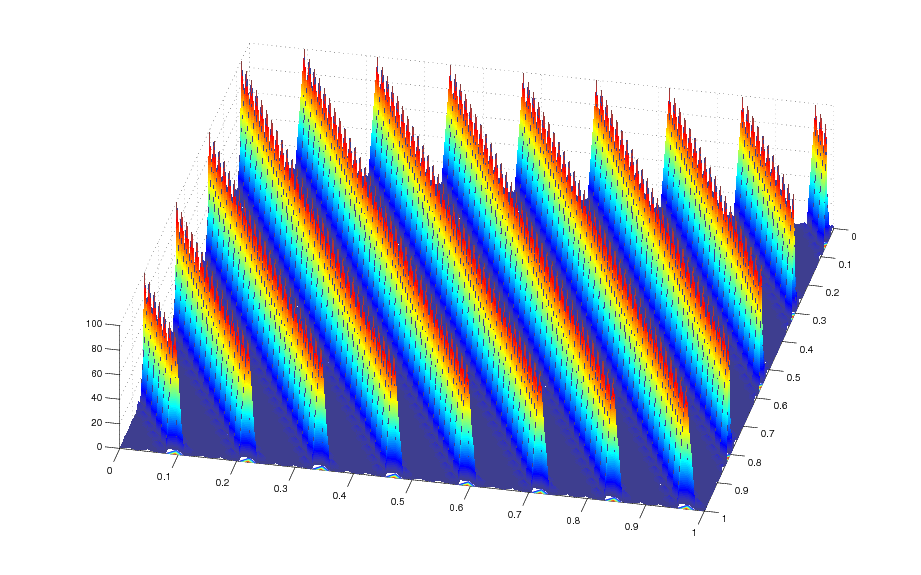
\includegraphics[width=6 in]{perm.eps}

Because of heterogeneity in the medium, the solution for velocity and saturatio are periodic.
Compare the following pictures on four meshes at time $t=T$:\\
Velocity-x:\\
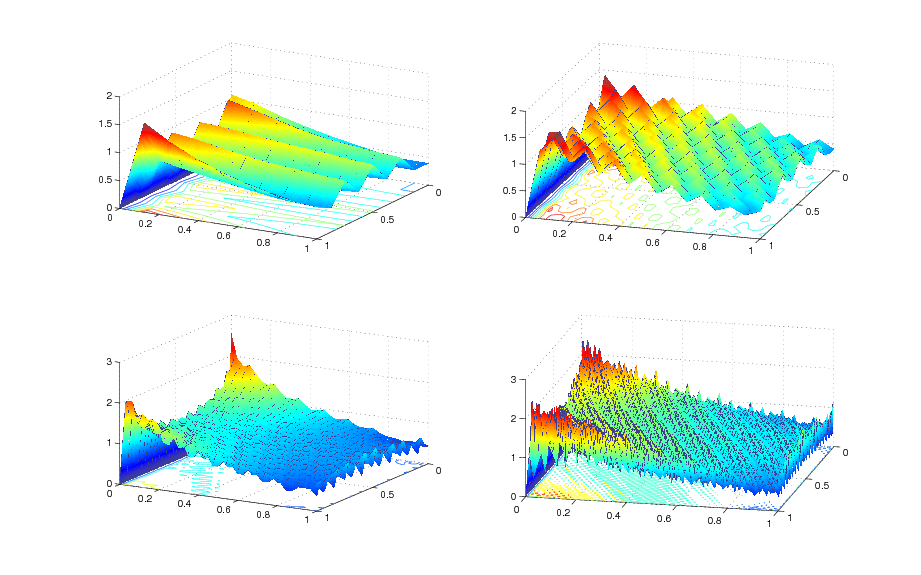
\includegraphics[width=5 in]{solu14meshes.eps}
\\
Velocity-y:\\
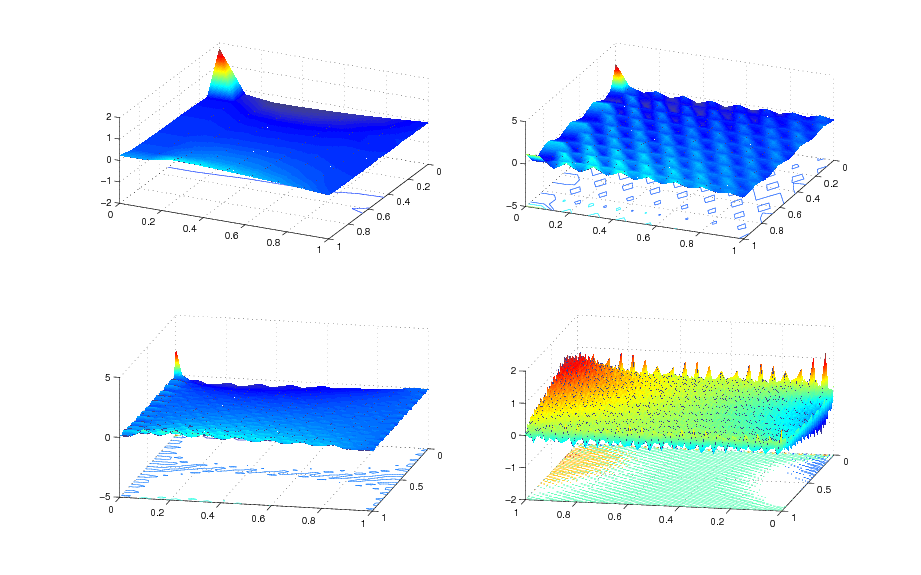
\includegraphics[width=5 in]{solu24meshes.eps}
\\
Pressure:\\
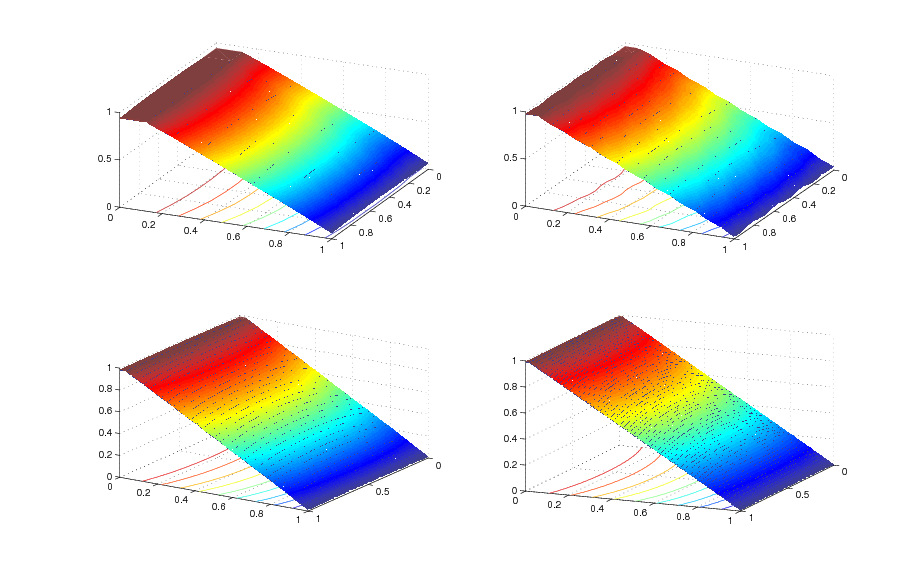
\includegraphics[width=5 in]{solp4meshes.eps}
\\
Saturation:\\
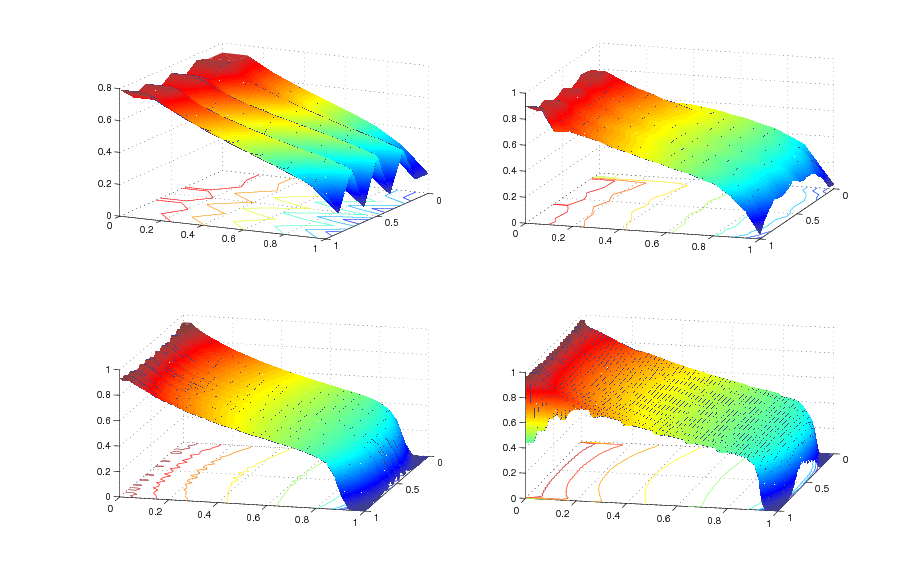
\includegraphics[width=5 in]{sols4meshes.eps}
\\
From above comparation, we can see pressure is stable but velocity and saturation are not. 
The reason is heterogeneity of the medium and some complexity fo the dynamic systems.
By our direct numerical computation, only fine mesh solution is able to catch the subgrid properties.
That means an accurate well-posed computation requires tremendous amount of computer memory and CPU time. 
But usually ,it easily exceed the limit of today's computer resources.\\
There are some alternative approaches have been developed. A common approach is to "scale up" a heterogeneous medium. 
This method is to find an effective representation of permeablility on a coarse mesh so that the large scale flow can be correctly computed on this mesh.The computational cost is thus greatly reduced.
\\
At last,let's see Oil Production Rate on the boundary $\Gamma_{2}$:
$$ PR(t)=1-\frac{\int_{\Gamma_{2}} (\mathbf{u}\cdot \mathbf{n})F(S)dx}{\int_{\Gamma_{2}} (\mathbf{u} \cdot \mathbf{n})dx}$$

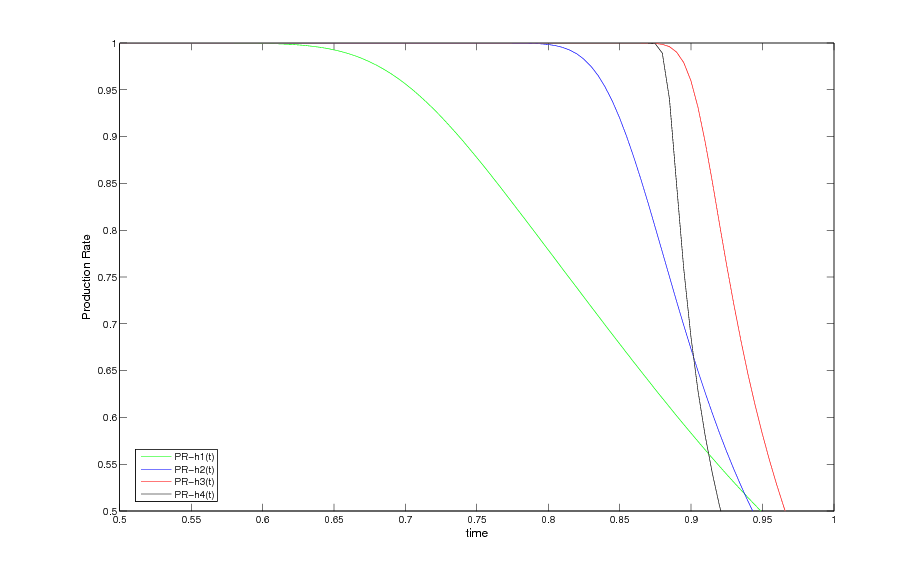
\includegraphics[width=6 in]{pr4meshes.eps}


\end{document}